\vspace{-0.15cm}
\section{Related works}
\vspace{-0.15cm}
\myparagraphnodot{Few-shot segmentation} aims to segment a target image given an annotated reference.
Early methods relied on compressed prototype representations~\cite{li2021adaptive, wang2019panet, lang2022learning, liu2022learning, fan2022self}, later replaced by attention- and correlation-based approaches~\cite{wang2020few, zhang2021few, moon2023msi, Min_2021_ICCV, hong2022cost} to better capture pixel-level relationships. More recently, research focused on leveraging the large-scale pretraining and generalization capabilities of vision foundation models \cite{zhu2024unleashing, zhang2023personalize, liu2023matcher, wang2023seggpt, xu2025hybrid}. 
Matcher \cite{liu2023matcher} and GF-SAM \cite{zhang2024bridge} utilize a training-free pipeline: DINOv2 extracts correspondences which are used to prompt SAM for segmentation. Similarly, VRP-SAM \cite{sun2024vrp} leverages a frozen SAM with an external encoder for feature matching. 
Recent works \cite{zhang2023personalize, zhu2024unleashing, meng2024segic} explore the use of \textit{a single VFM} \cite{bommasani2021opportunities} to jointly handle semantic understanding and mask prediction. DiffewS~\cite{zhu2024unleashing} exploit the emergent semantic correspondences in StableDiffusion \cite{rombach2022diffusion} to unify the process, while SegIC~\cite{meng2024segic} combines a frozen DINOv2 with a lightweight segmentation decoder. Yet, recent findings~\cite{zhang2023tale, zhang2024telling} suggest that diffusion and DINOv2 features offer complementary but disjoint strengths: the former offers spatial precision but weak semantics, the latter strong semantics but sparse matches. In contrast, we posit that \sam{} unifies both properties: its features possess high spatial granularity and implicitly encode semantic information. We show that this latent semantic structure can be extracted, effectively enabling FSS within a unified architecture.


\myparagraph{Semantic correspondences and Foundation Models}
Finding correspondences between images is a longstanding problem in Computer Vision  \cite{bay2006surf, lowe2004distinctive, kim2017fcss, rocco2018weakly, ofri2023neural}. While early deep-learning approaches train dedicated models to establish semantic correspondences \cite{kim2017fcss, rocco2018weakly}, recent works \cite{zhang2023tale, tang2023emergent} have shown that VFMs enable generalization across tasks \cite{tumanyan2022splicing, awais2025foundation, wei2024stronger, cuttano2025samwise}. Among them, DINOv2 \cite{oquab2023dinov2} and StableDiffusion \cite{rombach2022diffusion} have demonstrated a compelling ability to establish semantic correspondences between images \cite{zhang2023tale, ofri2023neural, zhang2024telling}.
Recently, Segment Anything 2 \cite{ravi2024sam} established itself as a foundation model for Video Object Segmentation. We observe that its pretraining, entailing matching object instances across frames under viewpoint changes and motion blur, closely parallels self-supervised learning frameworks \cite{yang2022inscon, yang2021instance, henaff2021efficient} that derive semantic understanding through self-similarity training. However, the extent to which \sam{} embeddings encode (if any) semantic concepts has not been studied yet. Recent applications in specialized domains \cite{zu2025medicalsam, bai2024medicalsam} utilize a frozen \sam{} in low-semantic-shift scenarios (\eg propagating masks across slices of 3D imagery given a support example). However, frozen \sam{} shows poor performance in standard FSS benchmarks requiring higher level semantic understanding. In this work, we shed light on this matter, providing insights into \sam{} feature structure and showing that semantic content can be disentanged from its embeddings.

\begin{figure*}[t]
\begin{center}
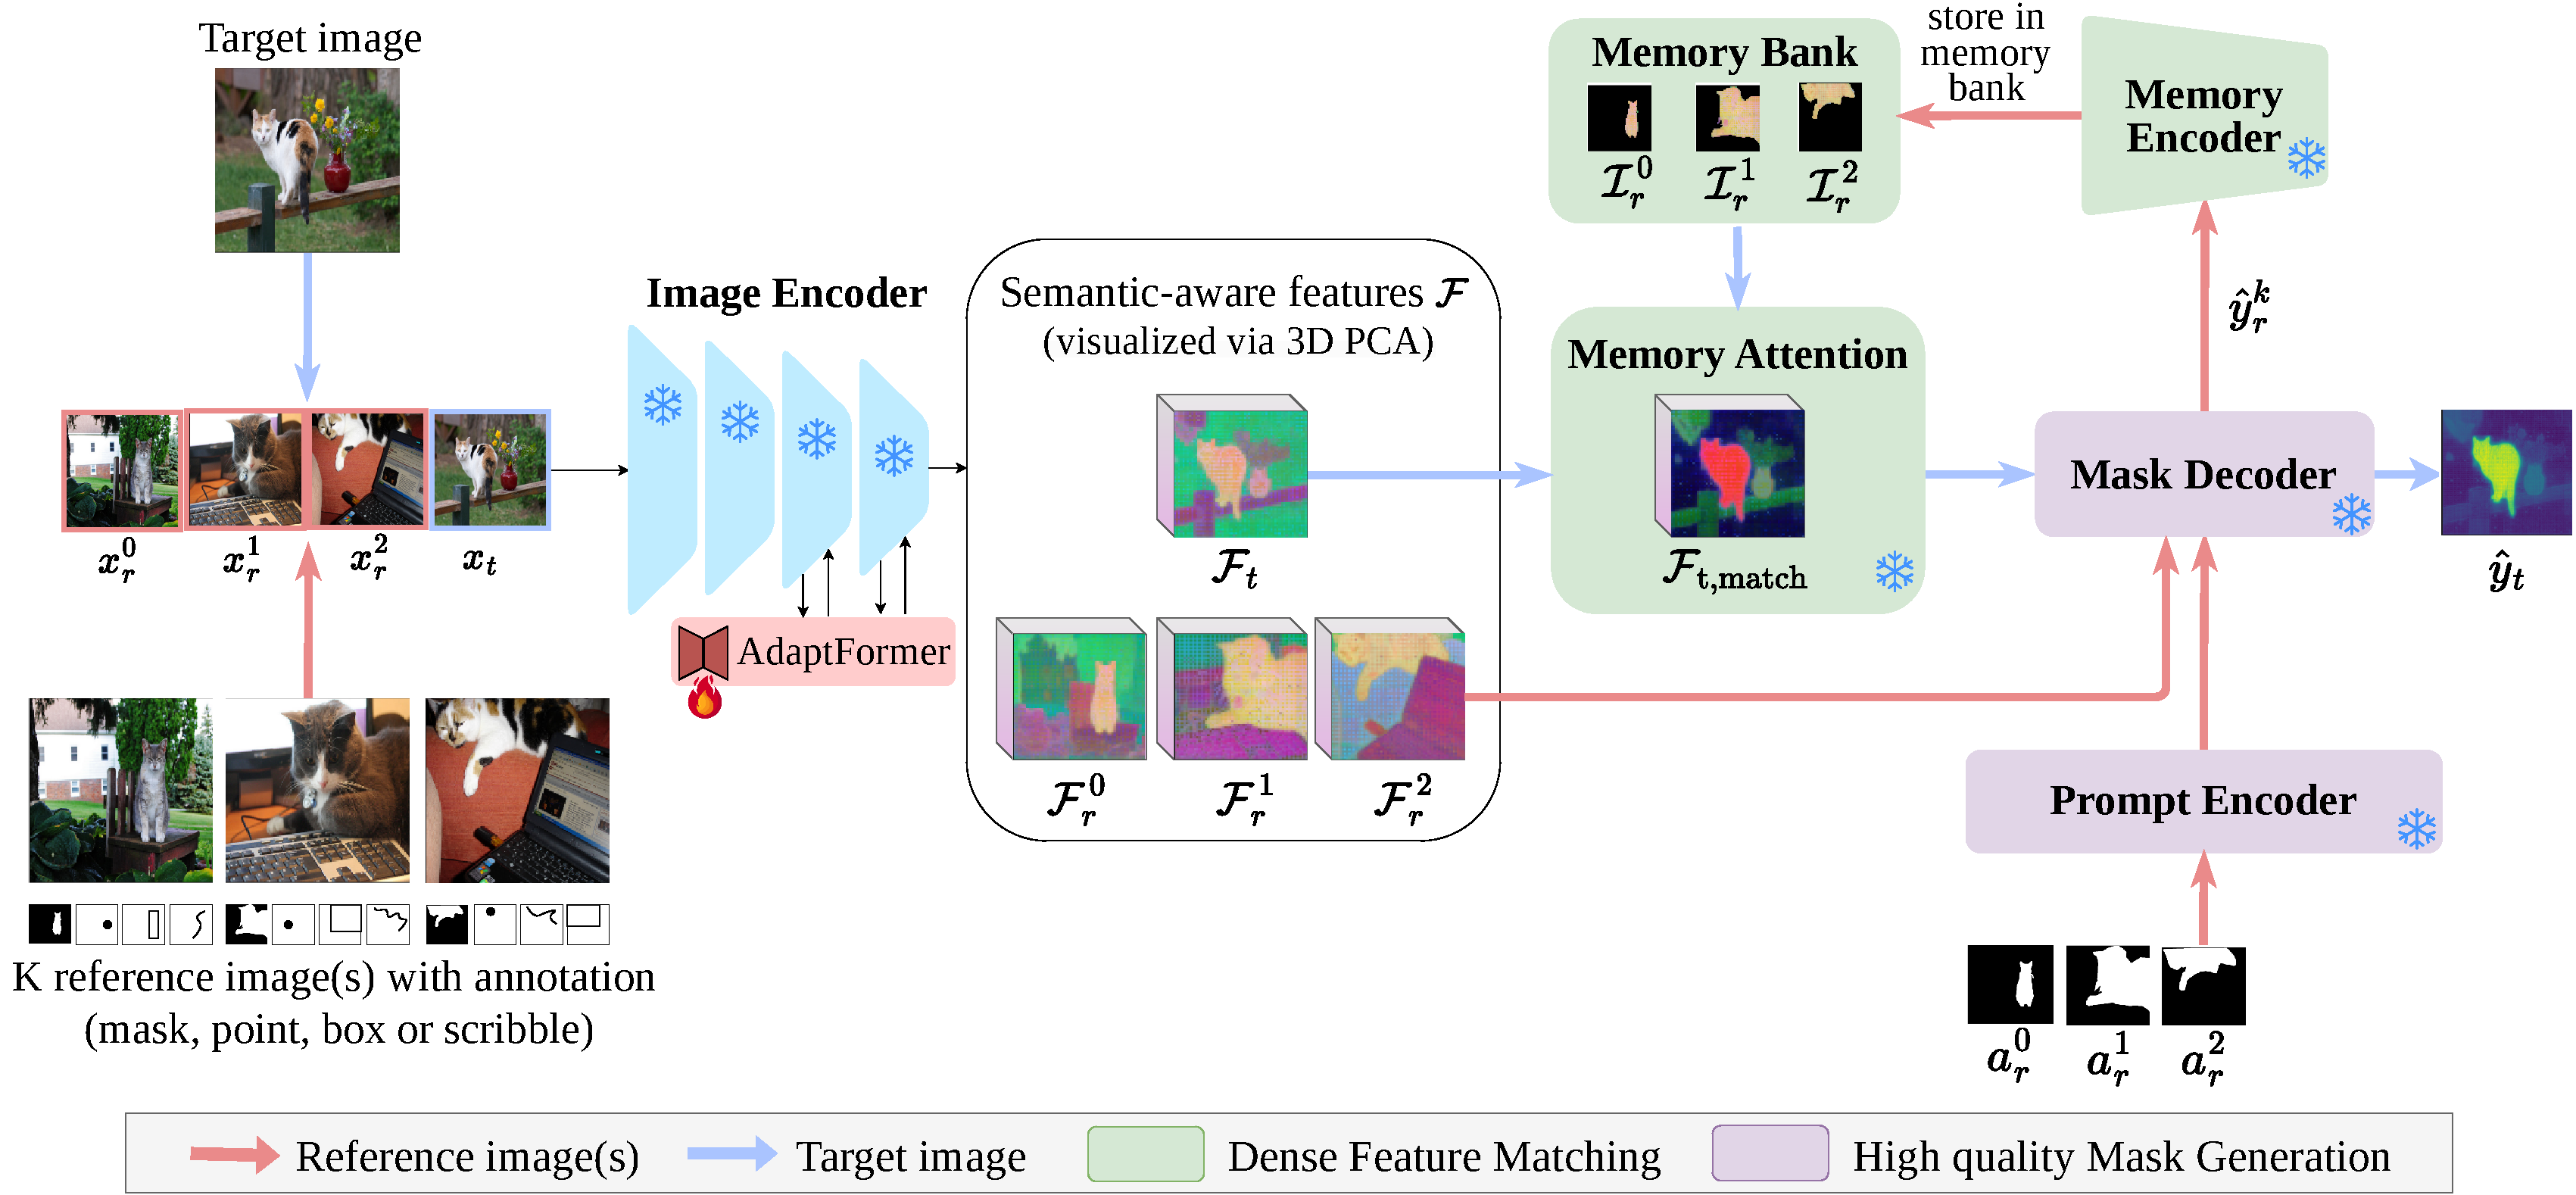
\includegraphics[width=\linewidth]{images/method.pdf}
\end{center}
\vspace{-0.2cm}
\caption{Overview of \textbf{\ours{}}: Given $k$ annotated reference images and a target image, we construct a pseudo-video by concatenating them, then leverage SAM2 streaming pipeline to process reference frames together with their annotations sequentially. 
We restructure \sam{} feature space to make its latent semantic structure \textit{explicit}, enabling mask propagation based on \textit{semantic similarity} from reference to target. The emergent semantic structure is visualized by the 3D PCA projection of $\mathcal{F}$.
}
\vspace{-0.2cm}
\label{fig:method}
\end{figure*}